Each Arabic letter represents a consonant, which means that short vowels are not
represented by the 36 characters, for this reason, the need of \textit{diacritics}
rises. \textit{Diacritics} are symbols that comes after a letter to state the
short vowel accompanied by that letter. There are four diacritics \textarabic{◌َ} \textarabic{◌ُ}
\textarabic{◌ِ} \textarabic{◌ْ} which represent the following short vowels
/\textit{a}/, /\textit{u}/, /\textit{i}/ and \textit{no-vowel} respectively,
their names are \textit{fat-ha, dam-ma, kas-ra and sukun} respectively.  The first
three symbols are called \textit{harakat}. Table \ref{tables:diacritics_dal}
shows the 4 diacritics on a letter.



% table: dal with diacritics
\begin{table}[H]
	\centering
	\begin{tabular}{c c c c c c}
		%\hline
		\toprule
		\textbf{\small{Diacritics}}     & \small{\textit{without}} & \small{\textit{fat-ha}} &
		\small{\textit{kas-ra}} & \small{\textit{dam-ma}} & \small{\textit{sukun}}\\
		%\hline
		\midrule
		\textbf{\small{Shape}}   & \textarabic{د} & \textarabic{دَ} & \textarabic{دِ} &
		\textarabic{دُ} & \textarabic{دْ}\\
		%\hline
		\bottomrule
	\end{tabular}
	\caption{Diacritics on the letter  \textarabic{ د }}\label{tables:diacritics_dal}
\end{table}



There are two more sub-diacritics made up of the basic four to represent two
cases:
\begin{definition}\label{def:shadaa_definition}
  \textbf{Shadaa}  \hfill \\
to indicate the letter is doubled. Any letter with
shaddah (\textarabic{ ّ } ) the letter should be duplicated: first letter with a
constant (sukoon) and second letter with a vowel (haraka) \cite{Alnagdawi2013}; Table  \ref{tables:shadda_dal}
shows the dal with shadda and the original letters.
% table: dal with shadda

\begin{table}[H]
	\centering
	\begin{tabular}{c c c}
		%\hline
		\toprule
		\textbf{\small{Diacritics}} & \small{\textit{letter with Shadda }} & \small{\textit{letters without shadaa  }} \\
		%\hline
		\midrule
		\textbf{\small{Shape}}  & \textarabic{دَّ} &  \textarabic{دْدَ}\\
		%\hline
		\bottomrule
	\end{tabular}
	\caption{Shadaa diacritics on the letter  \textarabic{ د }}\label{tables:shadda_dal}
\end{table}

\end{definition}

\begin{definition}\label{def:tanween_definition}
  \textbf{Tanween} \hfill \\
  %%% \ref{defa} and \ref{defb}
  is doubling the short vowel, and can convert
Tanween fathah, Tanween dhammah or Tanween kasrah by
replacing it with the appropriate vowel ( ُ◌ – dhammah, َ◌ –
fathah or ِ◌ –kasrah ) then add the Noon letter with constant to the end of the word \cite{Alnagdawi2013}. Table \ref{tables:Tanween_dal}
shows the difference between the original letter and the letter with Tanween

\begin{table}[H]
	\centering
	\begin{tabular}{c c c}
		%\hline
		\toprule
		\textbf{\small{Diacritics}} & \small{\textit{letter with tanween }} & \small{\textit{letters without tanween}} \\
		%\hline
		\midrule

          \textbf{\small{Tanween Fat-ha}}  & \textarabic{دً} &  \textarabic{دَ+نْ}\\
          \textbf{\small{Tanween Dam-ma}}  & \textarabic{دٌ} &  \textarabic{دُ+نْ}\\
          \textbf{\small{Tanween Kas-ra}}  & \textarabic{دٍ} &  \textarabic{دِ+نْ}\\


		\bottomrule
	\end{tabular}
	\caption{Tanween diacritics on the letter  \textarabic{ د }} \label{tables:Tanween_dal}
\end{table}


\end{definition}

 Arabs pronounce the sound \textit{/n/} accompanied \textit{sukun} at the end the indefinite words, that sound corresponds to this
letter \textarabic{نْ}, it is called \textit{noon-sakinah}, however, it is
just a phone, it is not a part of the indefinite word, if a word comes as a
definite word, no additional sound is added. Since it is not an essential sound,
it is not written as a letter, but it is written as  \textit{tanween}
\textarabic{◌ٌ ◌ً ◌ٍ}.
% adding tanween and its relationship to the previous letter
\textit{Tanween} states the sound \textit{noon-sakinah}, but as you have noticed,
there are 3 \textit{tanween} symbols, this because  \textit{tanween} is added as
a diacritic over the last letter of the indefinite word, one of the 3 harakat\textit{harakat} accompanies the last letter, the last letter's \textit{harakah}
needs to be stated in addition to the sound \textit{noon-sakinah}, so
\textit{tanween} is doubling the last letter's \textit{haraka}, this way the last
letter's \textit{haraka} is preserved in addition to stating the sound
\textit{noon-sakinah}; for example, \textarabic{رَجُلُ + نْ} is written
\textarabic{رَجُلٌ} and  \textarabic{رَجُلِ + نْ} is written \textarabic{رَجُلٍ}.


Those two definition, Definition ~\ref{def:shadaa_definition} and Definition ~\ref{def:tanween_definition}  will help us to reduce the dimension of the letter's feature vector as we will see in \textit{preparing data} section.


Diacritics makes short vowels clearer, but they are not necessary.
Moreover, a phrase without full diacritics or with just some on some letters is
right linguistically, so it is allowed to drop them from the text.

% Diacritics in Unicode
In Unicode, Arabic diacritics are standalone symbols, each of them has its own
unicode. This is in contrast to the Latin diacritics; e.g., in the set
\textit{\{ê, é, è, ë, ē, ĕ, ě\}}, each combination of the letter \textit{e} and a diacritic is represented by one unicode.

\newpage

\section{Arabic Arud Science}
% @@@ add el3elal and zahafat
% @@@ add tent picture
% @@@ add details into every bahr



\begin{definition}\label{def:arud}
  \textbf{Arud} \hfill \\
  In Arabic Arud natively has many meanings (the way, the direction, the light clouds and Mecca and Madinah \footnote{\textit{Mecca and Madinah are two cities in  Saudi Arabia}.}\cite{AlQuaed}. Arud is the science which studies The Arabic Poem meters and the rules which confirm if the Poem is sound meters \& broken meters. If we need to su
\end{definition}
 
The Author of this science is \textit{Al-Farahidi} (718 – 786 CE) has analyzed the
Arabic poetry; then he came up with that the succession of consonants and vowels
produce patterns or \textit{meters}, which make the music of poetry. He was one of the famous people who know The melodies and the musical parts of speech. He has
counted them fifteen meters.  After that, a student of \textit{Al-Farahidi} has
added one more meter to make them sixteen. Arabs call meters \textarabic{بحور}
which means "\textit{seas}" Poets have written poems without knowing exactly what rules which make a collection of words a poem.

The Reasons which makes \textit{Al-Farahidi} put this science is

  \begin{itemize}
  \item Protect the Arabic Poems from the broken meters.
  \item Distinguish between the original Arabic Poem and the non-poem or from the prose.
    \item Make the rules clear and easy for anyone who needs to write a poem.
  \end{itemize}

  Some people said that the one-day Al-Farahidi was walking into the metal-market and he was said some of the poems and for some reasons the knock of the metals matched the musical sound of the poem he was saying then he got an idea to explore the Arud of the poems.

 There are many reason for this science name 
  \begin{itemize}
  \item It named Arud because some people said he put this science in Arud place \textarabic{العَروض} \textit{with fat-ha, not with dam-ma such as the science name \textarabic{العُروض} } between Mecca and Al-Ta'if\cite{AlQuaed}.
  \item Arud in Arabic is noun come from verb \textarabic{يعرض} which means here to be assessed. They said because of Any poem should be assessed by Al-Arud science so, it named Al-Arud \cite{Alkafi1994}.
  \end{itemize}
  
  

  
    \newpage
    \subsection{Al-Farahidi and Pattern Recognition}
    This subsection is our opinion in Al-Farahidi and his method he followed during working on Arabic Poem Classifications.

\begin{enumerate}


\item Al-Farahidi thought there is a pattern for every collection of the poem by chance; however, He scientifically worked into this problem. He started analyzing the poem and add every group with the same tafa'il to the same class.
\item He analyzed the outliers and the particular case from every class and added it to his model.
\item He revised the Bohor and get the cases and generalize his case to be fit into all Poems.
\item His student once he found some Poems which weren't fit into any model to be a model for a new class.

\end{enumerate}
The best essential point which made us admired by Al-Farahidi is his way of research and his passion for getting an indeed succession model. Also, his model is general and followed all the steps currently any Data scientist follows to explore new pattern. Some people state that He died when he was thinking about the problem he hit a wall which made trouble for him. His die story shows that he was thinking in profoundly about this problem. One of the most interest thing I found during this research is how he found this pattern and Al-Farahidi’s way to find a new thing.
%@@@ add about student for sebayeah
%@@@ التأكد من أن القرآن والحديث ليس شعر وﻹن تصادف فهو ليس قصداً والشعر يجب أن يكون وزناً إتفاقاً

    \newpage
    
    \subsection{Feet Representation}
    A meter is an ordered sequence of feet. Feet are the basic
units of meters; there are ten of them.
\begin{definition}\label{def:feet}
  \textbf{Feet} \hfill \\  A Foot consists of
a sequence of \textbf{Sukun} (Consonants) represented as (0) and \textbf{Harakah} (Vowels) (/). Traditionally, feet are represented by mnemonic words called tafa’il \textarabic{تفاعيل}.
\end{definition}

Feets consists of three parts (Asbab (means Reasons in English) \textarabic{أسباب}, Awtaad (means Wedges in English) \textarabic{وتد}, Fawasel (means Breaks in English) \textarabic{فواصل}).
\begin{itemize}
\item \textbf{Reasons (\textarabic{أسباب})}: It has two types
  \begin{enumerate}
  \item \textbf{Light (\textarabic{سبب خفيف})} which happens when we have the first letter is harakah and the second is sukun (/0) example (\textarabic{هَبْ, لَمْ}).
    \item \textbf{Heavy (\textarabic{سبب ثقيل})} which happens when we have two harakah letter (//) example (\textarabic{لَكَ, بِكَ}).
    \end{enumerate}
    \item \textbf{Wedge (\textarabic{وتد})}: It has two types
  \begin{enumerate}
  \item \textbf{Combined Wedge (\textarabic{وتد مجموع})} which happens when we have two harakah letters followed by sukun (//0) example (\textarabic{مَشَى, عَلَى}).
    \item \textbf{Separated Wedge (\textarabic{وتد مفروق})} which happens when we have two harakah and in between a sukun letter (/0/) example (\textarabic{مُنْذُ, مِصْرُ}).
    \end{enumerate}
    \item \textbf{Breaks (\textarabic{فواصل}}): It has two types
  \begin{enumerate}
  \item \textbf{Small Break (\textarabic{فاصلة صغرى}}) which happens when we have three harakah letters followed by a sukun letter (///0) example (\textarabic{ذَهَبُوا, سُفُناً}).
    \item \textbf{Big Break (\textarabic{فاصلة كبرى}}) which happens when we have four harakah letters followed by a sukun letter  (////0) example (\textarabic{جَعَلَهُمْ}).\footnote{\textit{Some of Arab linguistic scientist assume the small Breaks as a combination between big reason and small reason. Same for the Big Breaks assumed to be a combination between Big reason and Combined Wedge. So, they didn't assume we have three types of feet it is only pure two and any other feets constructed from this two. In this thesis we assume there are three feets }.}
    \end{enumerate}
  \end{itemize}

\newpage
  \subsubsection{Rules for Arabic Letters Representation}
  Arabic Arud has one general rule in the poem representation which is we represent only the letters which is (spoken) not the written which means the letters with phonatics not the written. We have give the below rules as a results of the general rule.

  \begin{itemize}
  \item Any letter with \textit{harakah} represented as (/).
  \item Any letter with \textit{sukun} represented as (0).
  \item Any letter with shaddah represented by two letters the first one will be \textit{sukun} and the second letter will be \textit{harakah} represented as (0/) example (\textarabic{مُحَمََّد}) will be (//0//0).
  \item Any letter with tanween represented by two letters the first one is \textit{haraka} (/) and the second is \textit{sukun}.
  \item Alef without hamze (\textarabic{همزة الوصل}) and Wow Algmaa are not represented example (\textarabic{وُاعلَموا}) will be (/0//0)
  \item If we have a letter which is not written but (spoken) so, we will represent it example (\textarabic{هذا}) it include Alef but not written (\textarabic{هاذا}) the representation will be (/0/0).
  \item If we have \textit{Meem Aljamaa} with harakah so, it represented with \textit{Mad} example (\textarabic{هُمُ}) will be (//0) .
  \item \textit{Alef Mad} (\textarabic{آ}) will be two letters \textit{Alef with harakah} and \textit{Alef with sukun} example (\textarabic{آدَمُ}) will be (/0//).
    \item if the verse ended with \textit{harkah} we will add \textit{sukun} to it.


    \end{itemize}
Example: (note: the below representation first line is simliar the second one but with Arud language style ).
\begin{Arabic}
  \begin{traditionalpoem*}

    أرَاكَ عَصِيَّ الدّمعِ شِيمَتُكَ الصّبرُ، *** أما للهوى نهيٌ عليكَ ولا أمرُ ؟
     أرَاكَ عَصيْيَ دّمعِ شِيمَتُكَ صّبرُو، ***  أما للهوى نهينْ عليكَ ولا أمرو ؟
    
	\end{traditionalpoem*}
\end{Arabic}
%@@@ add example the difference between arud writting and the actual writing
\newpage

\subsection{Arabic Poetry Feets}

Arabic poetry feets has ten tafa'il \textarabic{تفاعيل} (scansion)  any peom constructed from these feets. They are eight from writing (syntax) perspective, But it ten in the rules.
\begin{savenotes}

\begin{table}[H]
  \centering
  \begin{tabular}{|c|c|c|c|}
    \hline
    \textbf{\#} & \textbf{Feet} & \textbf{Scansion} & \textbf{Construction} \\
    \hline
    1 & \textarabic{فَعُولُنْ}  & \texttt{0/0//} & combined wedge (\textarabic{فعو}) and small reason (\textarabic{لن})   \\
    2 &\textarabic{مَفاعِيلُنْ}& \texttt{0/0/0//} & combined wedge (\textarabic{مفا}) and two light reasons (\textarabic{عي}) (\textarabic{لن})   \\
    3 &\textarabic{مُفَاعَلَتُنْ}& \texttt{0///0//}  &    combined wedge (\textarabic{مفا}), heavy reason (\textarabic{عل}) and light reason (\textarabic{تن}) \\
    4 &\textarabic{فَاعِلاَتُنْ} & \texttt{0/0//0/}   & light reason (\textarabic{فا}), combined wedge (\textarabic{علا}) and light reason (\textarabic{تن})   \\
    5 &\textarabic{فَاعِ لاتُنْ} & \texttt{0/0//0/}  &  Separated wedge (\textarabic{فاع}) and two light reason (\textarabic{لا})(\textarabic{تن}) \footnote{\textit{We separated the letters (\textarabic{ع}) and (\textarabic{لا}) in (\textarabic{فاع لاتن}) to show that this part is separated wedge and distinguish between this feet  and (\textarabic{فاع لاتن}) which contains combined wedge  }.}  \\
    6 &\textarabic{فَاعِلُنْ}  & \texttt{0//0/}   & light reason (\textarabic{فا}) and combined wedge (\textarabic{علن})\\
    7 &\textarabic{مُتَفَاعِلُنْ}& \texttt{0//0///}  & heavy reason (\textarabic{مت}), light reason (\textarabic{فا}) and combined wedge (\textarabic{علن})  \\
    8 &\textarabic{مَفْعُولاَت} & \texttt{0//0///}   & two light reason (\textarabic{مف})(\textarabic{عو}) and separated wedge (\textarabic{لات}) \\
    9 &\textarabic{مُسْتَفْعِلُنْ} & \texttt{0//0/0/}  &  two light reason (\textarabic{مس})(\textarabic{تف}) and combination wedge (\textarabic{علن}) \\
    10 &\textarabic{مُسْتَفْعِ لُنْ} & \texttt{0//0/0/}  & light reason (\textarabic{مس}), separated wedge  (\textarabic{تفع}) and light reason  (\textarabic{لن})\footnote{\textit{We separated the letters (\textarabic{ع}) and (\textarabic{ل}) in (\textarabic{مستفع لن}) to show that it ends with a separated wedge and distinguish between this feet  and (\textarabic{مستفعلن}) which contains combined wedge }}\\


    \hline
  \end{tabular}
  \caption{The ten feet of the Arabic meters. }\label{arud:feet}
\end{table}
    \end{savenotes}

%% Every digit (\texttt{/} or \texttt{0}) represents
%%    the corresponding diacritic over a letter in the feet. \texttt{/} corresponds to
%%    a\textit{harakah} ( \textarabic{◌َ}, \textarabic{◌ُ}, or \textarabic{◌ِ}) and \texttt{0}
%%    corresponds to a \textit{sukun} (\textarabic{◌ْ}). Any \textit{mad} (\textarabic{و, ا, ى}) is
%%    equivalent to \texttt{0}, \textit{tanween} is equivalent to \texttt{0/}, and \textit{shaddah} is
%%    equivalent to \texttt{/0}%

    \newpage
\begin{definition}\label{def:meter}
  \textbf{Meter} \hfill \\
  %%%% What is rtythm,feet
  Poetic meters define the basic rhythm of the poem. Each meter is described by a set of ordered feet which can
be represented as ordered sets of consonants and vowels \cite{Almuhareb2015}.

% \textbf{Some conventions and terminologies}:

% What are poems and terminologies?
% What does a poem look like? bayt, shatr, ....
\begin{Arabic}
	\begin{traditionalpoem*}
          ولد الهدى فالكائنات ضياء *** وفم الزمان تبسم وثناء انشاء
          الروح والملأ الملائك حوله *** للدين والدنيا به بشراء

	\end{traditionalpoem*}
\end{Arabic}%



\end{definition}


\begin{definition}\label{def:verse}
  \textbf{Arabic Verse} \hfill \\ refers to "poetry" as contrasted to prose. Where the common unit of a verse is based on meter or rhyme, the common unit of prose is purely grammatical, such as a sentence or paragraph \footnote{\textit{ https://en.wikipedia.org/wiki/Verse\_(poetry)}.}. A verse know as \textit{Bayt} in Arabic \textarabic{بيت}

\end{definition}


\begin{definition}\label{def:shatr}
  \textbf{Shatr} \hfill \\  A verse consists of two halves, each of them is called \textit{shatr} and carries the full meter.  We will use the term \textit{shatr} to refer to a verse's half; whether the right or the left half.
\end{definition}



\begin{definition}\label{def:poem}
  \textbf{Poem} \hfill \\
  is a set of verses has the same meter and rhyme.

\end{definition}


\newpage

\subsection{Arabic Poetry Meters}

\subsubsection{Al-Taweel \textarabic{الطويل}}
\textbf{Why it named Al-Taweel?}
\textit{Al-Taweel is named Al-Taweel for two reasons; first, It is the longest meter between all meters. Second, It starts with Wedge then Reasons and Wedge is longer than Reasons. So, it named Al-Taweel. We need here to note later in the encoding section we will pad all other meters by zeros to make it all the same length. Example if the max Bayt is 82 so, any Bayt less than 82 will be padded by zeros to have the same length.\cite{Alkafi1994}
  }\\

\textbf{tafa'il}

\begin{Arabic}
	\begin{traditionalpoem*}
          فعلون مفاعيلن فعولن مفاعلن *** فعولن مفاعيلن فعولن مفاعيلن


	\end{traditionalpoem*}
      \end{Arabic}

\textbf{Example:}
\begin{Arabic}
	\begin{traditionalpoem*}
    %$> العصر العباسي >> ابن الفارض
          إذا جادَ أقوامٌ بِمالٍ رأيْتَهُمْ  *** يَجودونَ بالأرواحِ مِنْهُم بِلا بُخلِ
          //0/0 //0/0/0 //0/0 //0//0 *** //0/0 //0/0/0 //0/0 //0/0/0
          فعلون مفاعيلن فعولن مفاعلن *** فعولن مفاعيلن فعولن مفاعيلن

	\end{traditionalpoem*}
      \end{Arabic}

% % % 	% % % % % % % % % % % % % % % % % % % % % % % % % % % % % % % % % % % % % % % % % % % %

\subsubsection{Al-Madeed \textarabic{المديد}}
\textbf{Why it named Al-Madeed?}

\textit{Al-Madeed is named because of the reasons \textarabic{الأسباب} is represented in all its seven parts of tafa'il, One in the first part and the other in the second part. So, it named Madeed \textarabic{مديداً}\cite{Alkafi1994}
  }\\

% @@@note to add references

\textbf{tafa'il}

\begin{Arabic}
	\begin{traditionalpoem*}
فاعلاتن فاعلِن فاعلاتن *** فاعلاتن فاعلن فاعلاتن


	\end{traditionalpoem*}
      \end{Arabic}


\textbf{Example:}

\begin{Arabic}
	\begin{traditionalpoem*}
    % % % العصر الجاهلي >> المهلهل بن ربيعة - الزير
    يَا لِبَكْرٍ أَنْشِرُوا لِي كُلَيْباً	يَا لِبَكْرٍ أَيْنَ أَيْنَ الْفِرَارُ
/0//0/0 /0//0 /0//0/0 *** /0//0/0 /0//0 /0//0/0
فاعلاتن فاعلِن فاعلاتن *** فاعلاتن فاعلن فاعلاتن

	\end{traditionalpoem*}
      \end{Arabic}
\newpage



% % % 	% % % % % % % % % % % % % % % % % % % % % % % % % % % % % % % % % % % % % % % % % % % %

%@@@ check bohor name is same for all latex files
\subsubsection{Al-Baseet \textarabic{البسيط}}

\textbf{Why it named Al-Baseet?}
Al-Baseet there is a different idea behind this name
\begin{itemize}
\item The Reasons \textarabic{الأسباب} expanded into it is tafa'il. So, We will find at the beginning of every part two reasons so; it named Al-Baseet.
\item The other reasons which may be the more logic are the harkat  \textarabic{الحركات} expanded in its tafa'il.\cite{Alkafi1994}
  
\end{itemize}



\textbf{tafa'il}

\begin{Arabic}
	\begin{traditionalpoem*}
مستفعلن فعلن مستفعلن فاعلن *** مستفعلن فاعلن مستفعلن فاعلن


	\end{traditionalpoem*}
      \end{Arabic}


\textbf{Example:}

\begin{Arabic}
	\begin{traditionalpoem*}
          % % % العصر الجاهلي >> المهلهل بن ربيعة - الزير

لَيْسَ الجَمَال بأَثْوابٍ تُزَيِّنُنَا    ***	إن الجمال جمال العلم والأدب
/0/0//0 ///0 /0/0//0 ///0   ***  /0/0//0 ///0 /0/0//0 ///0
مستفعلن فعلن مستفعلن فاعلن  *** مستفعلن فاعلن مستفعلن فاعلن
	\end{traditionalpoem*}
      \end{Arabic}

% % % % % % % % % % % % % % % % % % % % % % % % % % % % % % % % % % % % % % % % % % % % % % %
\subsubsection{Al-Wafer \textarabic{الوافر}}
\textbf{Why it named Al-Wafer?}
Al-Wafer there are different ideas behind this name
\begin{itemize}
\item There is much harakat in its parts because there is no tafa'il has part includes harakat more than the word \textarabic{مفاعلتن}.
\item There are many parts to its base.\cite{Alkafi1994}
\end{itemize}

\textbf{tafa'il}

\begin{Arabic}
	\begin{traditionalpoem*}

          مفاعلتن مفاعلتن مفاعلتن *** مفاعلتن مفاعلتن مفاعلتن

	\end{traditionalpoem*}
      \end{Arabic}


\textbf{Example:}

\begin{Arabic}
  \begin{traditionalpoem*}
    %%% الأولى >> العصر الجاهلي >> عمرو بن كلثوم >> أَلاَ هُبِّي بِصَحْنِكِ فَاصْبَحِيْنَا ( معلقة )
    إِذَا بَلَـغَ الفِطَـامَ لَنَا صَبِـيٌّ *** تَخِـرُّ لَهُ الجَبَـابِرُ سَاجِديْنَـا
    //0///0 //0///0 //0/0 ***  //0///0 //0///0 //0/0
    مفاعلتن مفاعلتن فعولن  *** مفاعلتن مفاعلتن فعولن

	\end{traditionalpoem*}
      \end{Arabic}
\newpage

% % % % % % % % % % % % % % % % % % % % % % % % % % % % % % % % % % % % % % % % % % % % % % %

\subsubsection{Al-Kamel \textarabic{الكامل}}
\textbf{Why it named Al-Kamel?}
\textit{Al-Kamel is named because its harakat is fully integrated and it is 30 harakah which is not similar to any other Bahr has this numbers of harakat. However, Al-wafer has much harakat in its parts but not the same number as Al-Kamel. Al-Wafer has the harakat but it not overwritten into its source but Al-Kamel it is written into its source \textarabic{أصله}. So, Al-Kamel in Arabic named due to it is more integrated  \textarabic{أكمل} than Al-Wafer \cite{Alkafi1994}.
}\\

\textbf{tafa'il}

\begin{Arabic}
	\begin{traditionalpoem*}
متفاعلن متفاعلن متفاعلن *** متفاعلن متفاعلن متفاعلن


	\end{traditionalpoem*}
      \end{Arabic}


\textbf{Example:}

\begin{Arabic}
	\begin{traditionalpoem*}
    % % % الأولى >> العصر الجاهلي >> عنترة بن شداد >> هلْ غادرَ الشُّعراءُ منْ متردَّم ( معلقة )
وَلَقَدْ شَفَا نَفْسِي وَأَبْرَأَ سُقْمَهَا *** قِيلُ الفَوَارِسِ وَيكَ عَنْتَرَ أَقْدِمِ
///0//0 /0/0//0 ///0//0 ***  /0/0//0 ///0//0 ///0//0
متفاعلن مستفعلن متفاعلن *** مستفعلن متفاعلن متفاعلن

	\end{traditionalpoem*}
      \end{Arabic}

% % % % % % % % % % % % % % % % % % % % % % % % % % % % % % % % % % % % % % % % % % % % % % %

\subsubsection{Al-Hazaj \textarabic{الهزج}}
\textbf{Why it named Al-Hazaj?}
\textit{Al-Hazaj is named because of the sound reverberation in its parts. Al-Hazaj in Arabic is sound frequency. So, due to the sound reverberation, it named AL-Hazaj. Also, Because every part ends for two reasons so, it made some of sound like a piece of music to be Al-Hazaj \cite{Alkafi1994}.  }\\

\textbf{tafa'il}

\begin{Arabic}
	\begin{traditionalpoem*}
مفاعيلن مفاعيلن *** مفاعيلن مفاعيلن


	\end{traditionalpoem*}
      \end{Arabic}


\textbf{Example:}

\begin{Arabic}
	\begin{traditionalpoem*}
%%%%أدب .. ابن عبد ربه
          أَيَا مَنْ لاَمَ في الحُبِّ *** وَلَمْ يَعْلَمْ جَوى قَلبي
          //0/0/0 //0/0/0 *** //0/0/0 //0/0/0
          مفاعيلن مفاعيلن *** مفاعيلن مفاعيلن




	\end{traditionalpoem*}
      \end{Arabic}


% % % % % % % % % % % % % % % % % % % % % % % % % % % % % % % % % % % % % % % % % % % % % % %

\subsubsection{Al-Rejz \textarabic{الرجز}}
\textbf{Why it named Al-Rejz?}
\textit{Al-Rejz is named Al-Rezj because it constructed from three parts. If there is an animal and someone pull this animal by one leg and the animal walk into three legs in Arabic named Rejz \textarabic{رجزاً}, this is the reason it named Rejz because of it has three parts similar than animal pulled by one leg and walk into three legs. Also, in Arabic, if we have a camel when it stands up has some disturbances due to it sick or has any issue it named Rejz Camel \textarabic{جمل رجز}, and in Arabic disturbance \textarabic{إضطراب} means Rejz for example \cite{Alkafi1994}.}\\


\textbf{tafa'il}

\begin{Arabic}
  \begin{traditionalpoem*}
    مستفعلن مستفعلن مستفعلن *** مستفعلن مستفعلن مستفعل


	\end{traditionalpoem*}
      \end{Arabic}


\textbf{Example:}

\begin{Arabic}
  \begin{traditionalpoem*}
    دار لسلمى إذ سليمى جارة *** قفر ترى آيانها مثل الزّبر
    /0/0//0 /0/0//0 /0/0//0 *** /0/0//0 /0/0//0 /0/0//0
مستفعلن مستفعلن مستفعلن *** مستفعلن مستفعلن مستفعلن



	\end{traditionalpoem*}
      \end{Arabic}
      % % % % % % % % % % % % % % % % % % % % % % % % % % % % % % % % % % % % % % % % % % % % % % %


\subsubsection{Al-Raml \textarabic{الرمل}}
\textbf{Why it named Al-Raml?}
\textit{Al-Raml is named Al-Raml because Al-Raml is a type of the singing which constructed from this Bahr. Another reason is the Wedges is appeared in between the Reasons so; it named Al-Raml due to the diversity between the Reasons and the wedges inside the tafa'il \cite{Alkafi1994}.}\\

\textbf{tafa'il}

\begin{Arabic}
  \begin{traditionalpoem*}

    فاعلاتن فاعلاتن فاعلاتن *** فاعلاتن فاعلاتن فاعلاتن


	\end{traditionalpoem*}
      \end{Arabic}


\textbf{Example:}

\begin{Arabic}
  \begin{traditionalpoem*}

    إنما الدنيا غرور كلها *** مثل لمغ اﻵل في أرض الفقار
    /0//0/0 /0//0/0 /0//0 *** /0//0/0 /0//0/0 /0//0/0
    فاعلاتن فاعلاتن فاعلن *** فاعلاتن فاعلاتن فاعلاتن


	\end{traditionalpoem*}
      \end{Arabic}


      % % % % % % % % % % % % % % % % % % % % % % % % % % % % % % % % % % % % % % % % % % % % % % %


\subsubsection{Al-Sarea \textarabic{السريع}}
\textbf{Why it named Al-Sarea?}
\textit{Al-Sarea is named Al-Sarea in Arabic Al-Sarea means the fastest. It named these because its speed in teste \textarabic{الزوق} or its parts\textarabic{التقطيع}. The other reason because its three parts have 7 reasons and the reasons are faster than the wedges.\cite{Alkafi1994}}\\

\textbf{tafa'il}

\begin{Arabic}
  \begin{traditionalpoem*}

مستفعلن مستفعلن مفعولات *** مستفعلن مستفعلن مفعولات

	\end{traditionalpoem*}
      \end{Arabic}


\textbf{Example:}

\begin{Arabic}
  \begin{traditionalpoem*}


    أزمان سلمى لا يرى مثلها الر *** راؤون في شام ولا عراق
/0/0//0 /0/0//0 /0//0 *** /0/0//0 /0/0//0 /0//00
مستفعلن مستفعلن مفعولات *** مستفعلن مستفعلن مفعولات



	\end{traditionalpoem*}
      \end{Arabic}



      % % % % % % % % % % % % % % % % % % % % % % % % % % % % % % % % % % % % % % % % % % % % % % %


\subsubsection{Al-Monsareh \textarabic{المنسرح}}
\textbf{Why it named Al-Monsareh?}
\textit{to be written later :) :) \cite{Alkafi1994}.}\\

\textbf{tafa'il}

\begin{Arabic}
  \begin{traditionalpoem*}

مستفعلن مفعولات مستفعلن *** مستفعلن مفعولات مستفعلن

	\end{traditionalpoem*}
      \end{Arabic}


\textbf{Example:}

\begin{Arabic}
  \begin{traditionalpoem*}

    إن ابن زيد لا زال مستعملا *** للخير يفشى فى مصره العرفا
    /0/0//0 /0/0/0/ /0/0//0 *** /0/0//0 /0/0/0/ /0///0
    مستفعلن مفعولات مستفعلن *** مستفعلن مفعولات مفتعلن



	\end{traditionalpoem*}
      \end{Arabic}


      \newpage
      % % % % % % % % % % % % % % % % % % % % % % % % % % % % % % % % % % % % % % % % % % % % % % %


\subsubsection{Al-Khafeef \textarabic{الخفيف}}
\textbf{Why it named Al-Khafeef?}
\textit{Al-Khafeef name in Arabic means light. The reason behind the name is its wedge last harkah connected to its reason so, it became light \textarabic{خفت}. The other reason is its light in teste \textarabic{الزوق} or its parts \textarabic{التقطيع} because it has a part with three reasons and the reasons are lighter than wedges\cite{Alkafi1994}. }\\

\textbf{tafa'il}

\begin{Arabic}
  \begin{traditionalpoem*}

    فاعلاتن مستفع لن فاعلاتن *** فاعلاتن مستفع لن فاعلاتن
    %%%%مستفع لن
	\end{traditionalpoem*}
      \end{Arabic}


\textbf{Example:}

\begin{Arabic}
  \begin{traditionalpoem*}


    حل أهلي ما بين دوني فبادو *** لى وحلّت علوية بالسخال
    /0//0/0 /0/0//0  /0//0/0 *** /0//0/0 /0/0//0 /0//0/0
    فاعلاتن مستفع لن فاعلاتن *** فاعلاتن مستفع لن فاعلاتن


	\end{traditionalpoem*}
      \end{Arabic}

            % % % % % % % % % % % % % % % % % % % % % % % % % % % % % % % % % % % % % % % % % % % % % % %


\subsubsection{Al-Modarea \textarabic{المضارع}}
\textbf{Why it named Al-Modarea?}
\textit{Al-Modarea in Arabic means the present. It named by this name because it is the present version of the Al-Hazaj. Also, This Bahr wasn't famous in Arabic Poem and there weren't any popular peams or poetry used this Bahr before \cite{Alkafi1994}. }\\

\textbf{tafa'il}

\begin{Arabic}
  \begin{traditionalpoem*}

مفاعلين فاع لاتن *** مفاعلين فاع لاتن

  \end{traditionalpoem*}
      \end{Arabic}


\textbf{Example:}

\begin{Arabic}
  \begin{traditionalpoem*}


    كأن لم يكن جديراً *** بحفظ الذي أضاعا
    //0/0/  /0//0/0 *** //0/0/  /0//0/0
    مفاعيل  فاع لاتن *** مفاعيل  فاع لاتن


	\end{traditionalpoem*}
      \end{Arabic}
 \newpage
            % % % % % % % % % % % % % % % % % % % % % % % % % % % % % % % % % % % % % % % % % % % % % % %


\subsubsection{Al-Moktadeb \textarabic{المقتضب}}
\textbf{Why it named Al-Moktadeb ?}
\textit{Al-Moktadeb in Arabic means reproduced from another thing \textarabic{الإقتطاع} and because this Bahr word is all appeared into Al-Monsareh in all its words but also there is a difference in the order of the parts. So, it named Al-Moktadeb because it seems to reproduce from Al-Monsareh. We will have another section which will focus on the relation between the Bohor \cite{Alkafi1994}.  % @@@note to add references of the section
}\\


\textbf{tafa'il}

\begin{Arabic}
  \begin{traditionalpoem*}

مفعولات مستفعلن *** مفعولات مستفعلن

  \end{traditionalpoem*}
      \end{Arabic}


\textbf{Example:}

\begin{Arabic}
  \begin{traditionalpoem*}

    حف كأسها الحبب *** فهي فضة ذهب
    /0//0/  /0///0 *** /0//0/  /0///0
    فاعلات  مفتعلن *** فاعلات مفتعلن




	\end{traditionalpoem*}
      \end{Arabic}

      % % % % % % % % % % % % % % % % % % % % % % % % % % % % % % % % % % % % % % % % % % % % % %


      

      \subsubsection{Al-Mojtaz \textarabic{المجتز}}
\textbf{Why it named Al-Mojtaz?}
\textit{Al-Mojtaz in Arabic name is similar meaning for Al-Moktadeb it means reproduced from another thing \textarabic{الإقتطاع أو الإجتزاز} and because these Bahr words are all appeared into Al-khafeef in all its words but also there is a difference in the order of the parts. So, it named Al-Mojtaz because it seems it reproduced from Al-khafeef \textarabic{إجتُزَّ من بحر الخفيف} \cite{Alkafi1994}.}\\


\textbf{tafa'il}

\begin{Arabic}
  \begin{traditionalpoem*}

    مستفع لن فاعلاتن *** مستفع لن فاعلاتن

	\end{traditionalpoem*}
      \end{Arabic}


\textbf{Example:}

\begin{Arabic}
  \begin{traditionalpoem*}


    أنت الذى ولدتك *** أسماء بنت الحباب
    /0/0//0  ///0/ *** /0/0//0  /0//0/0
    مستفع لن  فعِلاتُ *** مستفع لن فاعلاتن


	\end{traditionalpoem*}
      \end{Arabic}

      \newpage
                  % % % % % % % % % % % % % % % % % % % % % % % % % % % % % % % % % % % % % % % % % % % % % % %


\subsubsection{Al-Motaqareb \textarabic{المتقارب}}
\textbf{Why it named Al-Motaqareb?}
\textit{Al-Motaqareb in Arabic means convergent and is named by this name because the wedges are convergent to each other this is because between every two wedges one reason, so the wedges are convergent to each other. Also, another reason is its parts are similar to each other, so it named Al-Motaqareb \cite{Alkafi1994}.
}
\\

\textbf{tafa'il}

\begin{Arabic}
  \begin{traditionalpoem*}
    فعولن فعولن فعولن فعولن *** فعولن فعولن فعولن فعولن


	\end{traditionalpoem*}
      \end{Arabic}

%%%http://www.uobabylon.edu.iq/uobColeges/lecture_view.aspx?fid=19&depid=1&lcid=31904
\textbf{Example:}

\begin{Arabic}
  \begin{traditionalpoem*}

    فأمَّا تَميمٌ، تَميمُ بنُ مُرٍّ *** فألفاهُمُ القَومُ رَوْبَى، نِياما
    //0/0 //0/0 //0/0 //0/0 *** //0/0 //0/0 //0/0 //0/0
    فعولن فعولن فعولن فعولن *** فعولن فعولن فعولن فعولن




	\end{traditionalpoem*}
      \end{Arabic}

                        % % % % % % % % % % % % % % % % % % % % % % % % % % % % % % % % % % % % % % % % % % % % % % %


\subsubsection{Al-Motadarek \textarabic{المتدارك}}
\textbf{Why it named Al-Motadarek?}
There are different ideas behind this name.
\begin{itemize}
  \item Al-Motadarek in Arabic means explored because Al-Farahidi forgets this Bahr and his student Al-Akhfash Al-Awsat has explored it named by this name.
 %%@@@ (215/830)
  \item Al-Motadarek in Arabic also means followed by something \textarabic{يُدرك}, and because this Bahr came after Al-Motaqareb, it names Al-Motadarek \cite{Alkafi1994}.\\
  \end{itemize}

\textbf{tafa'il}

\begin{Arabic}
  \begin{traditionalpoem*}
فَاْعِلُنْ فَاْعِلُنْ فَاْعِلُنْ فَاْعِلُنْ *** فَاْعِلُنْ فَاْعِلُنْ فَاْعِلُنْ فَاْعِلُنْ
	\end{traditionalpoem*}
      \end{Arabic}

      \textbf{Example:}

\begin{Arabic}
 \begin{traditionalpoem*}
    لَمْ يَدَعْ مَنْ مَضَى لِلَّذِيْ قَدْ غَبَرْ *** فَضْلَ عِلْمٍ سَوَى أَخْذِهِ بِالأثَرْ
    /0//0 /0//0 /0//0 /0//0 *** /0//0 /0//0 /0//0 /0//0
    فَاْعِلُنْ فَاْعِلُنْ فَاْعِلُنْ فَاْعِلُنْ *** فَاْعِلُنْ فَاْعِلُنْ فَاْعِلُنْ فَاْعِلُنْ
 \end{traditionalpoem*}
\end{Arabic}
  
  % % % % % % % % % % % % % % % % % % % % % % % % % % % % % % % % % % % % % % % % % % % % % % % 
  % % % % % % % % % % % % % % % % % % % % % % % % % % % % % % % % % % % % % % % % % % % % % % % 
  \newpage
  \subsection{Bohor Relations}

Al-Arud classes have a relation between each other. In this section, we will explain in brief this relation between them, and we will demonstrate if the effect of these relations in Chapter~\ref{ch_results}. There are five groups of relationships between the classes. These relations shows built based on the similarity and the difference between them
  
  @@@replace figures by tikz
  
  \begin{itemize}
  \item \textbf{Al-Mokhtalef \textarabic{المُخْتَلِف}}: This group contains three classes Al-Taweel, Al-Madeed and Al-Baseet Figure~\ref{fig:Circle_Mokhtalef} shows this relation between them.

    \begin{figure}[H]
 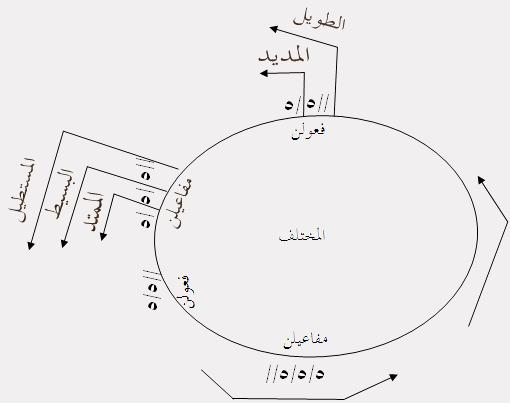
\includegraphics{./Figures/Ch_2_Background/Al-Mokhtalef.jpg}
 \caption{Al-Mokhtalef circle which contains three classes Al-Taweel, Al-Madeed and Al-Baseet}~\label{fig:Circle_Mokhtalef}
\end{figure}

\item \textbf{Al-Mo'talef \textarabic{المُؤْتَلِف}}: This group contains two classes Al-Kamel and Al-Wafer. Figure~\ref{fig:Circle_Motalef} shows this relation between them.

    \begin{figure}[H]
 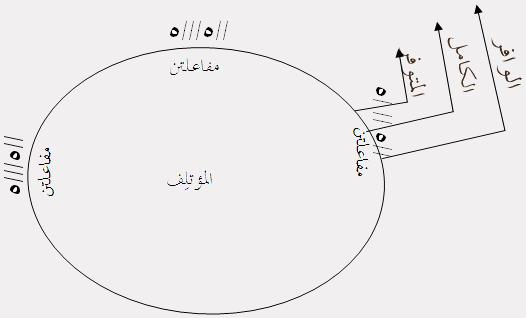
\includegraphics{./Figures/Ch_2_Background/Al-Mo'talef.jpg}
 \caption{Al-Mo'talef circle which contains three classes Al-Kamel and Al-Wafer}~\label{fig:Circle_Motalef}
\end{figure}


\item \textbf{Al-Mojtaleb \textarabic{المُجْتَلَب}}: This group contains three classes Al-Raml, Al-Rejz and Al-Hazaj. Figure~\ref{fig:Circle_Mojtaleb} shows this relation between them.

\begin{figure}[H]
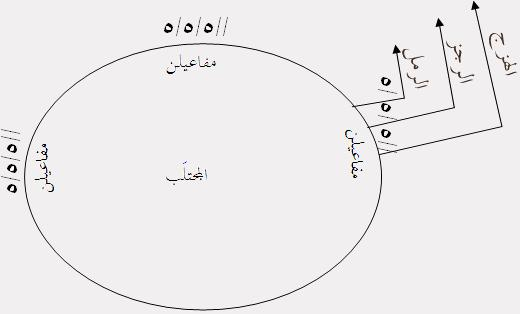
\includegraphics{./Figures/Ch_2_Background/Mojtaleb.jpg}
\caption{Al-Mojtaleb circle which contains three classes }~\label{fig:Circle_Mojtaleb}
\end{figure}


\item \textbf{Al-Moshtabeh \textarabic{المُشْتَبِه}}: This group contains six classes Al-Sarea, Al-Monsareh, Al-Khafeef, Al-Modarea, Al-Moktadeb and Al-Mojtaz. Figure~\ref{fig:Circle_AlMoshtabeh} shows this relation between them.

\begin{figure}[H]
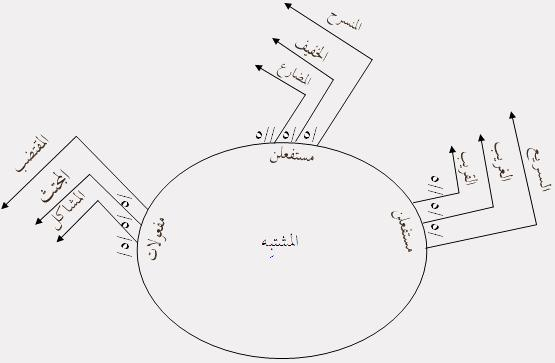
\includegraphics{./Figures/Ch_2_Background/Al-Moshtabeh.jpg}
\caption{Al-Moshtabeh circle which contains six classes Al-Sarea, Al-Monsareh, Al-Khafeef, Al-Modarea, Al-Moktadeb and Al-Mojtaz }~\label{fig:Circle_AlMoshtabeh}
\end{figure}


\item \textbf{Al-Motafeq \textarabic{المُتَّفِق}}: This group contains two classes Al-Motaqareb and Al-Motadarek. Figure~\ref{fig:Circle_Motafeq} shows this relation between them.

\begin{figure}[H]
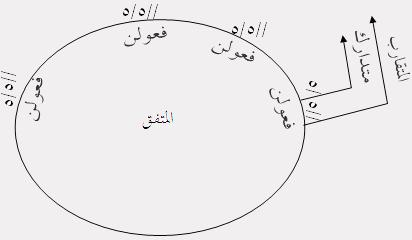
\includegraphics{./Figures/Ch_2_Background/Al-Motafeq.jpg}
\caption{Al-Motafeq circle which contains six classes Al-Motaqareb and Al-Motadarek}~\label{fig:Circle_Motafeq}
\end{figure}


\end{itemize}

\newpage


%%% Local Variables:
%%% mode: latex
%%% TeX-master: "../master"
%%% TeX-engine: xetex
%%% End:
